% S4 signal plot (Figure: signals). Generated by eval/plot_signals.py from eval/results/confidence_pilot.csv;
% do not edit by hand. Needs \usepackage{tikz}.
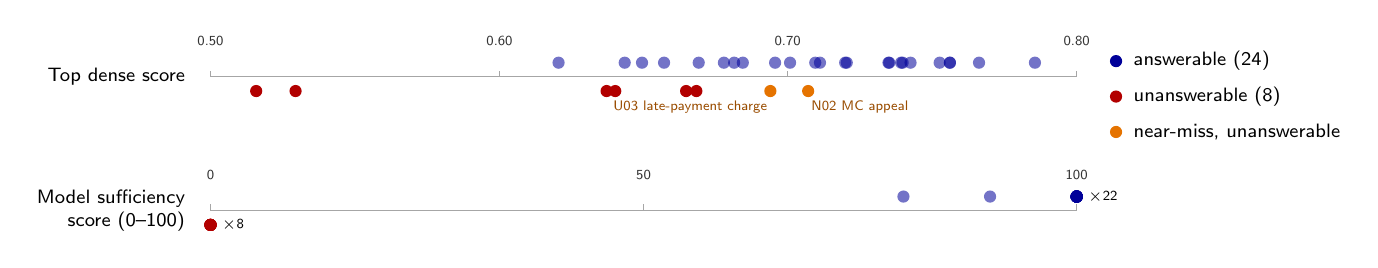
\begin{tikzpicture}[font=\sffamily\small]
  \node[anchor=east,font=\sffamily\scriptsize,align=right] at (-0.2,1.70) {Top dense score};
  \draw[gray!70] (0,1.70) -- (11.0,1.70);
  \draw[gray!70] (0.00,1.70) -- (0.00,1.78);
  \node[font=\sffamily\tiny,text=gray!40!black] at (0.00,2.15) {0.50};
  \draw[gray!70] (3.67,1.70) -- (3.67,1.78);
  \node[font=\sffamily\tiny,text=gray!40!black] at (3.67,2.15) {0.60};
  \draw[gray!70] (7.33,1.70) -- (7.33,1.78);
  \node[font=\sffamily\tiny,text=gray!40!black] at (7.33,2.15) {0.70};
  \draw[gray!70] (11.00,1.70) -- (11.00,1.78);
  \node[font=\sffamily\tiny,text=gray!40!black] at (11.00,2.15) {0.80};
  \fill[blue!60!black,opacity=0.55] (9.76,1.88) circle (2.2pt);
  \fill[blue!60!black,opacity=0.55] (8.77,1.88) circle (2.2pt);
  \fill[blue!60!black,opacity=0.55] (5.26,1.88) circle (2.2pt);
  \fill[blue!60!black,opacity=0.55] (8.62,1.88) circle (2.2pt);
  \fill[blue!60!black,opacity=0.55] (6.20,1.88) circle (2.2pt);
  \fill[blue!60!black,opacity=0.55] (9.26,1.88) circle (2.2pt);
  \fill[blue!60!black,opacity=0.55] (8.06,1.88) circle (2.2pt);
  \fill[blue!60!black,opacity=0.55] (10.47,1.88) circle (2.2pt);
  \fill[blue!60!black,opacity=0.55] (7.74,1.88) circle (2.2pt);
  \fill[blue!60!black,opacity=0.55] (5.48,1.88) circle (2.2pt);
  \fill[blue!60!black,opacity=0.55] (4.42,1.88) circle (2.2pt);
  \fill[blue!60!black,opacity=0.55] (6.76,1.88) circle (2.2pt);
  \fill[blue!60!black,opacity=0.55] (8.08,1.88) circle (2.2pt);
  \fill[blue!60!black,opacity=0.55] (8.79,1.88) circle (2.2pt);
  \fill[blue!60!black,opacity=0.55] (7.68,1.88) circle (2.2pt);
  \fill[blue!60!black,opacity=0.55] (9.39,1.88) circle (2.2pt);
  \fill[blue!60!black,opacity=0.55] (8.89,1.88) circle (2.2pt);
  \fill[blue!60!black,opacity=0.55] (9.39,1.88) circle (2.2pt);
  \fill[blue!60!black,opacity=0.55] (8.61,1.88) circle (2.2pt);
  \fill[blue!60!black,opacity=0.55] (5.76,1.88) circle (2.2pt);
  \fill[red!70!black] (0.58,1.52) circle (2.2pt);
  \fill[red!70!black] (5.03,1.52) circle (2.2pt);
  \fill[orange!90!black] (7.11,1.52) circle (2.2pt);
  \node[font=\sffamily\tiny,text=orange!60!black,anchor=north east,inner sep=1pt] at (7.11,1.44) {U03 late-payment charge};
  \fill[red!70!black] (6.17,1.52) circle (2.2pt);
  \fill[red!70!black] (1.08,1.52) circle (2.2pt);
  \fill[red!70!black] (6.04,1.52) circle (2.2pt);
  \fill[blue!60!black,opacity=0.55] (6.52,1.88) circle (2.2pt);
  \fill[blue!60!black,opacity=0.55] (7.36,1.88) circle (2.2pt);
  \fill[blue!60!black,opacity=0.55] (7.17,1.88) circle (2.2pt);
  \fill[blue!60!black,opacity=0.55] (6.65,1.88) circle (2.2pt);
  \fill[red!70!black] (5.14,1.52) circle (2.2pt);
  \fill[orange!90!black] (7.59,1.52) circle (2.2pt);
  \node[font=\sffamily\tiny,text=orange!60!black,anchor=north west,inner sep=1pt] at (7.59,1.44) {N02 MC appeal};
  \node[anchor=east,font=\sffamily\scriptsize,align=right] at (-0.2,0.00) {Model sufficiency\\score (0--100)};
  \draw[gray!70] (0,0.00) -- (11.0,0.00);
  \draw[gray!70] (0.00,0.00) -- (0.00,0.08);
  \node[font=\sffamily\tiny,text=gray!40!black] at (0.00,0.45) {0};
  \draw[gray!70] (5.50,0.00) -- (5.50,0.08);
  \node[font=\sffamily\tiny,text=gray!40!black] at (5.50,0.45) {50};
  \draw[gray!70] (11.00,0.00) -- (11.00,0.08);
  \node[font=\sffamily\tiny,text=gray!40!black] at (11.00,0.45) {100};
  \fill[blue!60!black,opacity=0.55] (11.00,0.18) circle (2.2pt);
  \fill[blue!60!black,opacity=0.55] (11.00,0.18) circle (2.2pt);
  \fill[blue!60!black,opacity=0.55] (11.00,0.18) circle (2.2pt);
  \fill[blue!60!black,opacity=0.55] (8.80,0.18) circle (2.2pt);
  \fill[blue!60!black,opacity=0.55] (9.90,0.18) circle (2.2pt);
  \fill[blue!60!black,opacity=0.55] (11.00,0.18) circle (2.2pt);
  \fill[blue!60!black,opacity=0.55] (11.00,0.18) circle (2.2pt);
  \fill[blue!60!black,opacity=0.55] (11.00,0.18) circle (2.2pt);
  \fill[blue!60!black,opacity=0.55] (11.00,0.18) circle (2.2pt);
  \fill[blue!60!black,opacity=0.55] (11.00,0.18) circle (2.2pt);
  \fill[blue!60!black,opacity=0.55] (11.00,0.18) circle (2.2pt);
  \fill[blue!60!black,opacity=0.55] (11.00,0.18) circle (2.2pt);
  \fill[blue!60!black,opacity=0.55] (11.00,0.18) circle (2.2pt);
  \fill[blue!60!black,opacity=0.55] (11.00,0.18) circle (2.2pt);
  \fill[blue!60!black,opacity=0.55] (11.00,0.18) circle (2.2pt);
  \fill[blue!60!black,opacity=0.55] (11.00,0.18) circle (2.2pt);
  \fill[blue!60!black,opacity=0.55] (11.00,0.18) circle (2.2pt);
  \fill[blue!60!black,opacity=0.55] (11.00,0.18) circle (2.2pt);
  \fill[blue!60!black,opacity=0.55] (11.00,0.18) circle (2.2pt);
  \fill[blue!60!black,opacity=0.55] (11.00,0.18) circle (2.2pt);
  \fill[red!70!black] (0.00,-0.18) circle (2.2pt);
  \fill[red!70!black] (0.00,-0.18) circle (2.2pt);
  \fill[red!70!black] (0.00,-0.18) circle (2.2pt);
  \fill[red!70!black] (0.00,-0.18) circle (2.2pt);
  \fill[red!70!black] (0.00,-0.18) circle (2.2pt);
  \fill[red!70!black] (0.00,-0.18) circle (2.2pt);
  \fill[blue!60!black,opacity=0.55] (11.00,0.18) circle (2.2pt);
  \fill[blue!60!black,opacity=0.55] (11.00,0.18) circle (2.2pt);
  \fill[blue!60!black,opacity=0.55] (11.00,0.18) circle (2.2pt);
  \fill[blue!60!black,opacity=0.55] (11.00,0.18) circle (2.2pt);
  \fill[red!70!black] (0.00,-0.18) circle (2.2pt);
  \fill[red!70!black] (0.00,-0.18) circle (2.2pt);
  \node[font=\sffamily\tiny,anchor=west,inner sep=1pt] at (11.10,0.18) {$\times$22};
  \node[font=\sffamily\tiny,anchor=west,inner sep=1pt] at (0.10,-0.18) {$\times$8};
  \fill[blue!60!black] (11.50,1.90) circle (2.2pt);
  \node[right,font=\sffamily\scriptsize] at (11.60,1.90) {answerable (24)};
  \fill[red!70!black] (11.50,1.45) circle (2.2pt);
  \node[right,font=\sffamily\scriptsize] at (11.60,1.45) {unanswerable (8)};
  \fill[orange!90!black] (11.50,1.00) circle (2.2pt);
  \node[right,font=\sffamily\scriptsize] at (11.60,1.00) {near-miss, unanswerable};
\end{tikzpicture}
